\chapter{Resultados}

\begin{figure}[H]
  \centering
  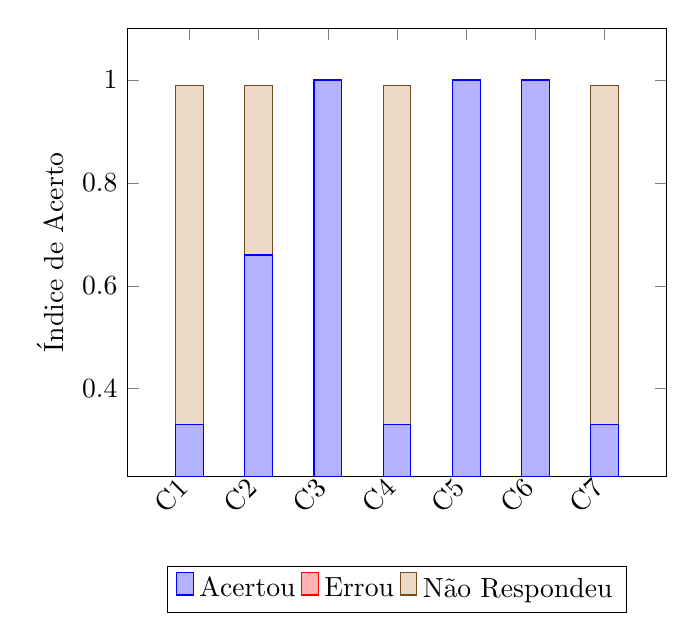
\begin{tikzpicture}
  \begin{axis}[
      ybar stacked,
      enlargelimits=0.15,
      legend style={at={(0.5,-0.20)},
        anchor=north,legend columns=-1},
      ylabel={Índice de Acerto},
      symbolic x coords={C1, C2, C3, C4, 
          C5, C6, C7},
      xtick=data,
      x tick label style={rotate=45,anchor=east},
      ]
  \addplot+[ybar] plot coordinates {(C1,0.33) (C2,0.66) 
    (C3,1) (C4,0.33) (C5,1) (C6,1) (C7,0.33)};
  \addplot+[ybar] plot coordinates {(C1,0) (C2,0) 
    (C3,0) (C4,0) (C5,0) (C6,0) (C7,0)};
  \addplot+[ybar] plot coordinates {(C1,0.66) (C2,0.33) 
    (C3,0) (C4,0.66) (C5,0) (C6,0) (C7,0.66)};
  \legend{Acertou, Errou, Não Respondeu}
  \end{axis}
  \end{tikzpicture}
  \caption{Índice de acerto sem o uso da ferramenta}
\end{figure}

\begin{figure}[H]
  \centering
  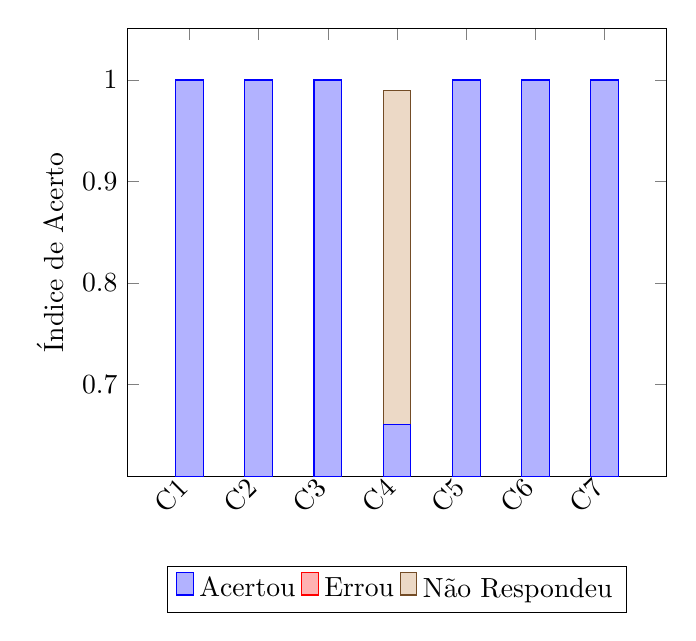
\begin{tikzpicture}
  \begin{axis}[
      ybar stacked,
      enlargelimits=0.15,
      legend style={at={(0.5,-0.20)},
        anchor=north,legend columns=-1},
      ylabel={Índice de Acerto},
      symbolic x coords={C1, C2, C3, C4, 
          C5, C6, C7},
      xtick=data,
      x tick label style={rotate=45,anchor=east},
      ]
  \addplot+[ybar] plot coordinates {(C1,1) (C2,1) 
    (C3,1) (C4,0.66) (C5,1) (C6,1) (C7,1)};
  \addplot+[ybar] plot coordinates {(C1,0) (C2,0) 
    (C3,0) (C4,0) (C5,0) (C6,0) (C7,0)};
  \addplot+[ybar] plot coordinates {(C1,0) (C2,0) 
    (C3,0) (C4,0.33) (C5,0) (C6,0) (C7,0)};
  \legend{Acertou, Errou, Não Respondeu}
  \end{axis}
  \end{tikzpicture}
  \caption{Índice de acerto com o uso da ferramenta}
\end{figure}

\begin{figure}[H]
  \centering
  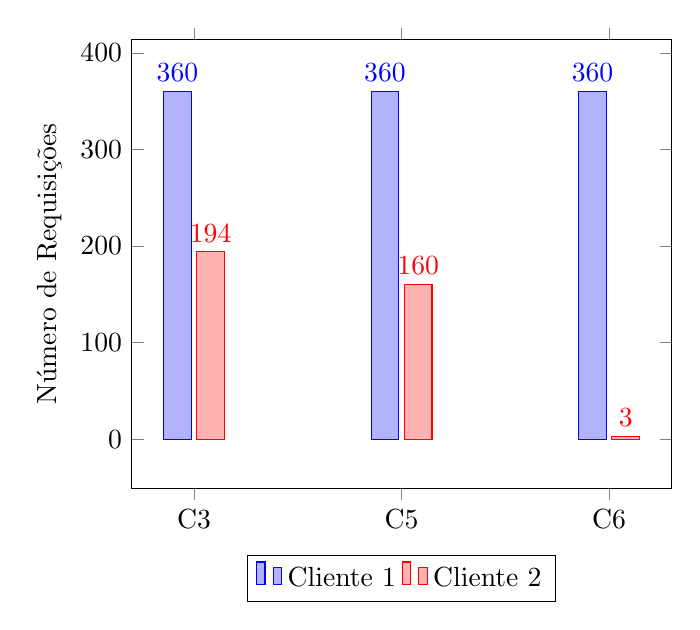
\begin{tikzpicture}
  \begin{axis}[
      ybar,
      enlargelimits=0.15,
      legend style={at={(0.5,-0.15)},
        anchor=north,legend columns=-1},
      ylabel={Número de Requisições},
      symbolic x coords={C3,C5,C6},
      xtick=data,
      nodes near coords,
      nodes near coords align={vertical},
      ]
  \addplot coordinates {(C3,360) (C5,360) (C6,360)};
  \addplot coordinates {(C3,194) (C5,160) (C6,3)};
  \legend{Cliente 1,Cliente 2}
  \end{axis}
  \end{tikzpicture}
  \caption{Comparação no número de requisições das mudanças OK}
\end{figure}

\begin{figure}[H]
  \centering
  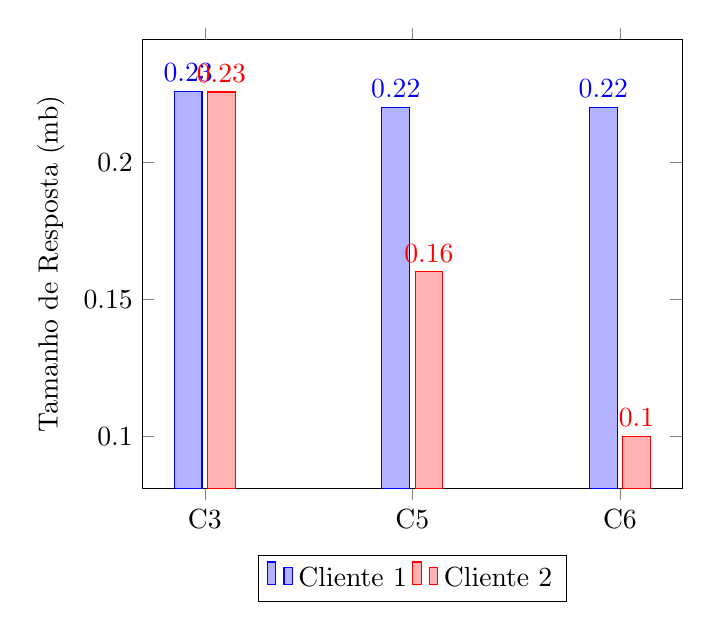
\begin{tikzpicture}
  \begin{axis}[
      ybar,
      enlargelimits=0.15,
      legend style={at={(0.5,-0.15)},
        anchor=north,legend columns=-1},
      ylabel={Tamanho de Resposta (mb)},
      symbolic x coords={C3,C5,C6},
      xtick=data,
      nodes near coords,
      nodes near coords align={vertical},
      ]
  \addplot coordinates {(C3,0.225777) (C5,0.22) (C6,0.22)};
  \addplot coordinates {(C3,0.225572) (C5,0.16) (C6,0.10)};
  \legend{Cliente 1,Cliente 2}
  \end{axis}
  \end{tikzpicture}
  \caption{Comparação no tamanho de resposta das mudanças OK}
\end{figure}

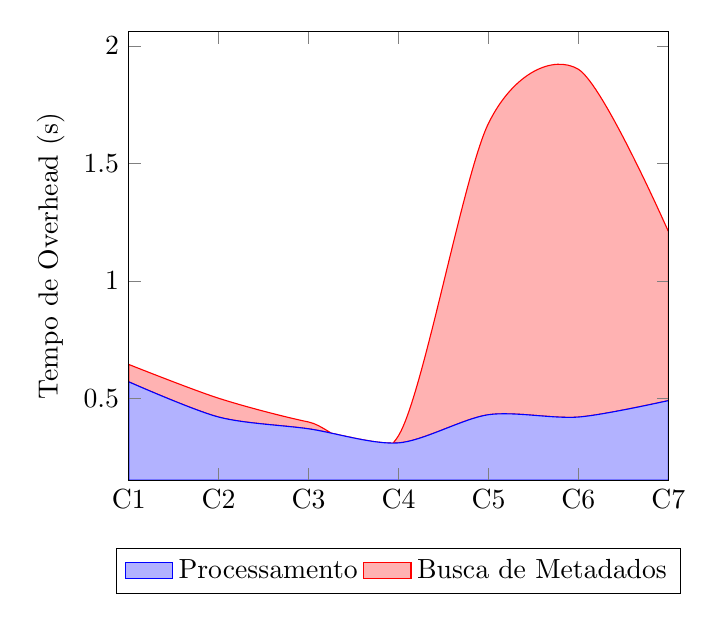
\begin{tikzpicture}
	\begin{axis}[
        ylabel={Tempo de Overhead (s)},
        legend style={at={(0.5,-0.15)},
        anchor=north,legend columns=-1},
		smooth,
		stack plots=y,
		area style,
        symbolic x coords={C1,C2,C3,C4,C5,C6,C7},
		enlarge x limits=false]
	\addplot coordinates
		{(C1,0.57) (C2,0.42) (C3,0.37) (C4,0.31) (C5,0.43) (C6,0.42) (C7,0.49)} 
		\closedcycle;
	\addplot coordinates
		{(C1,0.074) (C2,0.08) (C3,0.029) (C4,0.031) (C5,1.24) (C6,1.48) (C7,0.72)}
		\closedcycle;
    \legend{Processamento,Busca de Metadados}
	\end{axis}
\end{tikzpicture}
